\documentclass[11pt,letterpaper]{article}

%%%%%%%%%%%%%%%%%%%%%%%%%%%%%%%%%%%%%%%%%%%%%%%%%%%%%%%%%%%%%%%%%%%%%%%%%
\pagestyle{plain}                                                      %%
%%%%%%%%%% EXACT 1in MARGINS %%%%%%%                                   %%
\setlength{\textwidth}{6.5in}     %%                                   %%
\setlength{\oddsidemargin}{0in}   %% (It is recommended that you       %%
\setlength{\evensidemargin}{0in}  %%  not change these parameters,     %%
\setlength{\textheight}{8.5in}    %%  at the risk of having your       %%
\setlength{\topmargin}{0in}       %%  proposal dismissed on the basis  %%
\setlength{\headheight}{0in}      %%  of incorrect formatting!!!)      %%
\setlength{\headsep}{0in}         %%                                   %%
\setlength{\footskip}{.5in}       %%                                   %%
%%%%%%%%%%%%%%%%%%%%%%%%%%%%%%%%%%%%                                   %%
%\newcommand{\required}[1]{\section*{\hfil #1\hfil}}                    %%
\renewcommand{\refname}{\hfil References Cited\hfil}                   %%
%\bibliographystyle{plain}                                              %%
%%%%%%%%%%%%%%%%%%%%%%%%%%%%%%%%%%%%%%%%%%%%%%%%%%%%%%%%%%%%%%%%%%%%%%%%%

%PUT YOUR MACROS HERE

\usepackage{amsmath}
\usepackage{amsfonts}
\usepackage{amssymb}
\usepackage{graphicx}
\usepackage{ulem}
\usepackage[hidelinks]{hyperref}


\title{Muon Physics}


\author{Ian Hunt-Isaak\\ \begin{small}
Partner: Corina Miner
\end{small}}

\begin{document}


\date{}
\maketitle
\section*{1}
Corina turned in our piece.
\section*{2} %1
Consider the equation for the velocity of a point on a rotating circle of diameter d:
\begin{equation}
velocity = v\ (ft/min) * RPM = \pi \frac{d\ (in)}{12},
\end{equation}
where d is in inches and v is the tangent velocity.
Setting $v$ equal to the surface cutting speed, $d$ equal to tool diameter and using the approximation $\pi \approx \frac{2e}{\sqrt{3}} \approx 3$ we find
\begin{equation}
\label{eq:speed}
cuttingSpeed\ (sfm)= \frac{RPM*Tool Diameter\ (in)}{4}.
\end{equation}
As the cutting speed will be determined by the hardness of the material and the desired finish this equation is most useful in the following form:
\begin{equation}
\label{eq:RPM}
\frac{cuttingSpeed \times 4}{ToolDiameter} = RPM,
\end{equation}
which tells us what our spindle speed should be. 

The milling machine manual recommends a surface cutting speed of 60 (sfm) for stainless steel. Putting this into Eq. \ref{eq:RPM} we find that our RPM's should be set to $RPM = \frac{60 \times 4}{.5} = 480$ for milling stainless steel with 1/2" end mill. This is much slower than the 1700 RPMs that we used to machine our Aluminum block. This is because aluminum is a much softer metal and so can be cut more rapidly. In general the first considerations for the type of material should be meeting the required hardness, durability and other properties for the desired final piece. After those considering both cost and those limitations on specs it would be best to choose the easiest to machine material so that production of the object will be easy. If something requires a very hard or brittle metal then it could be difficult to machine and so it 

One could also use Eq. \ref{eq:speed} to calculate the max cutting speed to be used for a given RPM, though the cutting speed one should use would likely be lower once the properties of the material are taken into account. Doing that and setting our RPMs to the max on our machine of 1700 we find that $cuttingSpeed = \frac{1700 \times .5}{4} =212.5\ (sfm)$.
\section*{3} %2
My machining experience was overall a positive one. I began with more trepidation for use the tools such as the lathe than I left with. I gained a greater understanding of what is and isn't safe to do with the large tools. The second major part of the experience was learning not to rush as much as I might otherwise. Working to be both within tolerance and to have a nice finish forced me to be more considerate of my actions before I took them than I normally would have been. On the lathing section we lost a large amount of time due to confusion about how we were supposed to orient the tool. In working faster to regain the lost time we made a rougher than desired surface to the lathed piece. However this was partially resolved by applying sandpaper to the post. The other flaw in the quality of our pieces was the trench we milled, this was not done as smoothly as it could have been and there are clear markings on it, we should have made our cuts shallower. We were within tolerance for all things except the diameter of the post which was .03" under the acceptable range.
\section*{4} %3
The positioning of the tool relative to the piece is determined by whether the goal is to face or turn the piece. 
\section*{5} %3
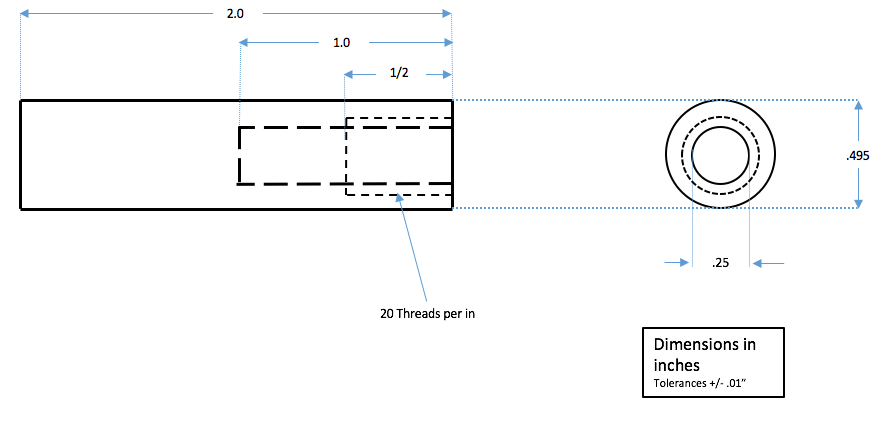
\includegraphics[width=\textwidth]{techDrawing.png}
\end{document}